\documentclass{siproblemset}

\usepackage{multicol}
\usepackage{xcolor}

% SI Session Information
\course{MTH 1321}
\sessionnum{8}
\sessiondate{2/25/21}

\warmup{Overview of Basic Derivative Rules}
\topic{Evaluating Derivatives}
\cooldown{Applications of the Derivative}

% Worksheet Information
\title{Product and Quotient Rules,\linebreak Rates of Change}
\sections{Section 3.3-3.4a}
\withnamespace

\begin{document}
    \maketitle
    
    \activity{Warmup}{Concept Review}{Try these problems \textbf{alone} as your peers join the session. Do your best to not refer to your notes.}{15 minutes}
    
    \mcq[2]{Evaluate the following:}{
        \task $\dddx \left[f(x)\cdot g(x)\right]$
        \task $\dddx \left[ \dfrac{f(x)}{g(x)}\right] $
    }
    \Tinysp
    
    \pagebreak
    \activity{Activity 1}{Computing Derivatives Using Derivative Rules}{Make a \textbf{group of two or three, all with the same colored worksheets,} to answer your assigned question. Try not to use your notes.}{30 minutes}

    \mcq{Compute the derivative.}{
        \task $f'(2),~~f(x)=x^3e^{x+2}$
        \Smallsp
        \task $\left[ (2x-9)\left(4e^x+1\right) \right]'$
        \Smallsp
        \task $f(x)=\dfrac{e^x}{x^2+1}$
        \Smallsp
        \task $f(x)=x^2(3+x^{-1})$
        \Smallsp
        \task $\dder[z]{t}\Bigr|_{t=3},~~z=\dfrac{-1}{10-t}$
        \Normalsp
        \task $\dddx\left[ \left(\sqrt x - 1\right)\left(\sqrt x + 1\right)\right] $
        \Smallsp
        \task $\left[x^{3/5}e^{5/3}\right]'$
        \Smallsp
        \task $g(u)=\dfrac{u+1}{e^u}$
        \Smallsp
    }\pagebreak

    \activity{Activity 2}{Derivatives From a Table}{Make a \textbf{{\em new} group of three, all with different colored worksheets,} to answer these questions. Try not to use your notes.}{30 minutes}

    \begin{multipartquestion}
        Use the following table to find the derivatives.
        
        \begin{center}
            \begin{tabular}{ |c|c|c|c| }
            	\hline
            	$f(3)$ & $f'(3)$ & $g(3)$ & $g'(3)$ \\ \hline
            	$5$    &   $3$   &  $-2$  &   $6$   \\ \hline
            \end{tabular}
        \end{center}
            
        \frq{$(fg)'(3)$}
        \Smallsp
        \frq{$(f/g)'(3)$}
        \Normalsp
        \frq{$\left[ (x+2)f(x)\right]'\Bigr|_{x=3} $}
        \pagebreak
        \frq{$G'(3)$ where $G(x)=(g(x))^2$}
        \Smallsp
        
    \end{multipartquestion}
    
    \activity{Cooldown}{Applications of the Derivative}{Attempt to do these problems \textbf{alone} then discuss your answers with the people around you.}{15 minutes}
    
    
    \frq{Find the points on the graph of the curve $y=\dfrac23x^3-5x-4$ at which the tangent line is parallel to $y=3x-2$}
    \Normalsp
    
    \frq{Draw the graph of $f'$ given the graph of $f$ below.}
    
    \begin{multicols}{2}
        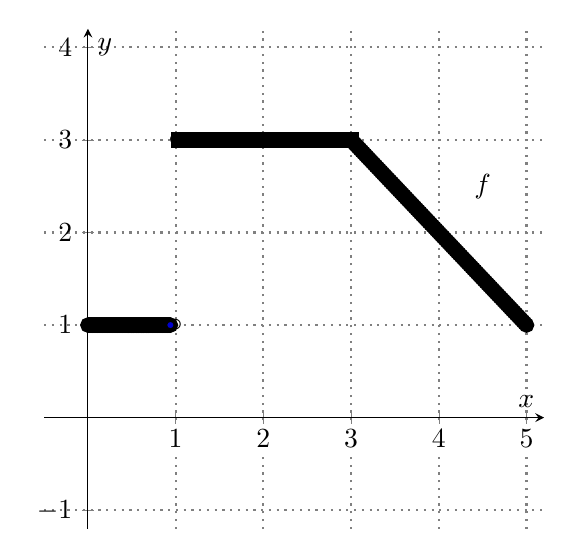
\begin{tikzpicture}
        \begin{axis}[axis x line=center, axis y line=middle,
        width=2.5in, height=2.5in, 
        scale only axis, %axis equal,
        xmin=-0.5, xmax=5.2,
        ymin=-1.2, ymax=4.2,
        xtick={0,...,5}, ytick={-1,...,4},
        xticklabel style={draw=none, inner sep=2pt, fill=white, text opacity=1},
        xlabel={$x$}, ylabel={$y$},
        grid=both, grid style={line width=.8pt, draw=gray, dotted},
        minor tick num=0, samples=100]
        \addplot+[black, ultra thick, domain=0:.94] {1};
        \addplot+[black, ultra thick, domain=1.03:3] {3};
        \addplot+[black, ultra thick, domain=3:5] {6-x};
        \node at (4.5,2.5) {$f$};
        \node at (1,1) {$\circ$};
        \node at (1,3) {$\circ$};
        \node at (3,3) {$\bullet$};
        \end{axis}
        \end{tikzpicture}
        
        \columnbreak
        
        \begin{tikzpicture}
        \begin{axis}[axis x line=center, axis y line=middle,
        width=2.5in, height=2.5in, 
        scale only axis, %axis equal,
        xmin=-0.5, xmax=5.2,
        ymin=-1.2, ymax=4.2,
        xtick={0,...,5}, ytick={-1,...,4},
        xticklabel style={draw=none, inner sep=2pt, fill=white, text opacity=1},
        xlabel={$x$}, ylabel={$y$},
        grid=both, grid style={line width=.8pt, draw=gray, dotted},
        minor tick num=0]
        \end{axis}
        \end{tikzpicture}
    \end{multicols}
%    \Tinysp
%    \frq{Draw the graph of $g$ given the graph of $g'$ below.}
%    
%    \begin{multicols}{2}
%        \begin{tikzpicture}
%        \begin{axis}[axis x line=center, axis y line=middle,
%        width=2.5in, height=2.5in, 
%        scale only axis, %axis equal,
%        xmin=-0.5, xmax=5.2,
%        ymin=-1.2, ymax=4.2,
%        xtick={0,...,5}, ytick={-1,...,4},
%        xticklabel style={draw=none, inner sep=2pt, fill=white, text opacity=1},
%        xlabel={$x$}, ylabel={$y$},
%        grid=both, grid style={line width=.8pt, draw=gray, dotted},
%        minor tick num=0, samples=100]
%        \addplot+[black, ultra thick, domain=0:.94] {1};
%        \addplot+[black, ultra thick, domain=1.03:3] {3};
%        \addplot+[black, ultra thick, domain=3:5] {6-x};
%        \node at (4.5,2.5) {$g'$};
%        \node at (1,1) {$\circ$};
%        \node at (1,3) {$\circ$};
%        \node at (3,3) {$\bullet$};
%        \end{axis}
%        \end{tikzpicture}
%        
%        \columnbreak
%        
%        \begin{tikzpicture}
%        \begin{axis}[axis x line=center, axis y line=middle,
%        width=2.5in, height=2.5in, 
%        scale only axis, %axis equal,
%        xmin=-0.5, xmax=5.2,
%        ymin=-1.2, ymax=4.2,
%        xtick={0,...,5}, ytick={-1,...,4},
%        xticklabel style={draw=none, inner sep=2pt, fill=white, text opacity=1},
%        xlabel={$x$}, ylabel={$y$},
%        grid=both, grid style={line width=.8pt, draw=gray, dotted},
%        minor tick num=0]
%        \end{axis}
%        \end{tikzpicture}
%    \end{multicols}
%    \mediumspace
\end{document}